\subsection{Selbsttestmodul im Lernprozess des Agenten}
\label{sec:Selbsttestmodul}

Das Selbsttestmodul ist ein essentielles Element unserer Systemarchitektur, welches die Schnittstelle zwischen Theorie und Praxis repräsentiert. Es bewertet und optimiert die Effektivität der vom Agenten erlernten Schaltstrategien.

\paragraph{Funktion und Notwendigkeit des Selbsttests}
Der Selbsttest bewertet die Schaltungsreaktionen auf definierte Testszenarien, um die Lernergebnisse des Agenten zu überprüfen, wie in Abbildung \ref{fig:RewardOverTime} dargestellt.
\begin{figure}[htbp]
    \centering
    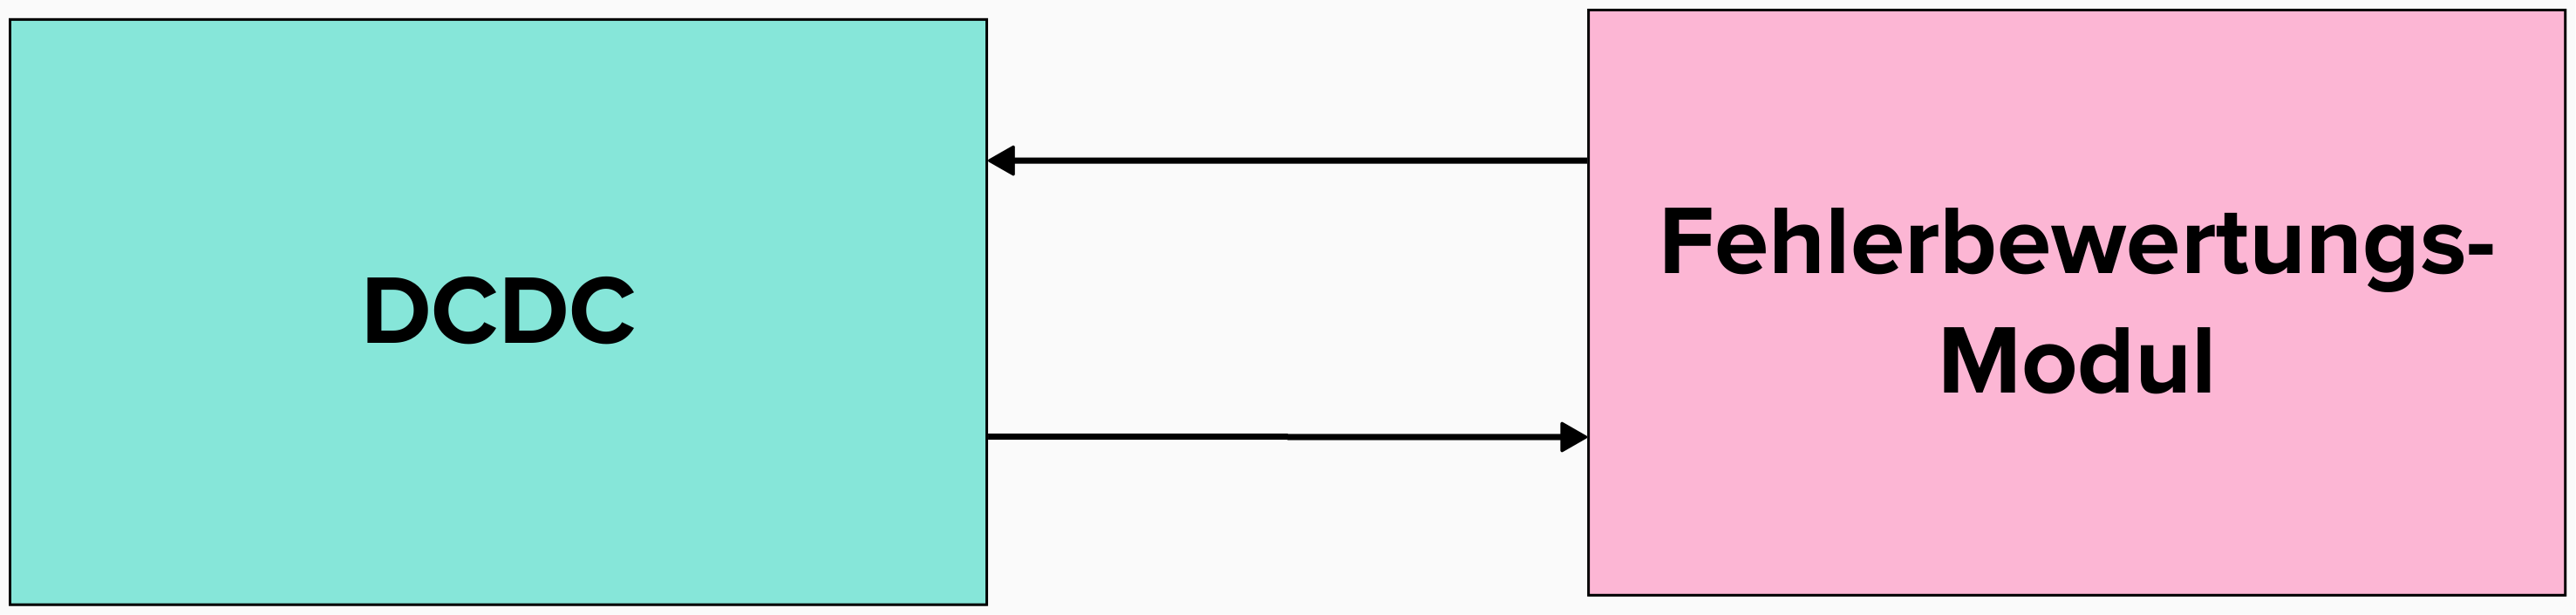
\includegraphics[width=0.5\linewidth]{3Experiment/2Experiment/4reward.png}
    \caption{Darstellung des Selbsttestmoduls im Regelkreis mit PID-Regler, PWM und DCDC-Konverter.}
    \label{fig:ControlLoop}
\end{figure}

\paragraph{Methodik der Performanzbewertung}
Die Bewertungsmethodik integriert die Abweichungen zwischen Soll- und Ist-Spannung, wobei größere Fehler durch Quadrierung stärker gewichtet werden. Extreme Spannungsspitzen werden, wie in Abbildung \ref{fig:CumulativeReward} gezeigt, exponentiell bestraft.
\begin{figure}[htbp]
    \centering
    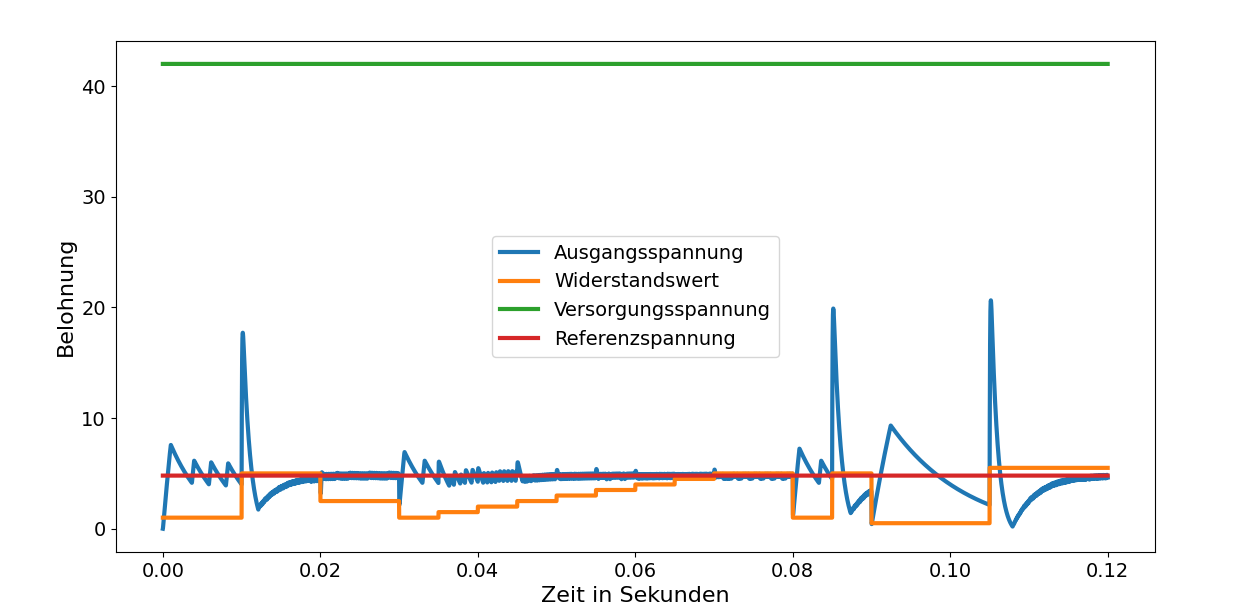
\includegraphics[width=0.99\linewidth]{3Experiment/2Experiment/4Reard_over_time.png.png}
    \caption{Visualisierung des Rewards über die Zeit während der Simulation.}
    \label{fig:RewardOverTime}
\end{figure}
\begin{figure}[htbp]
    \centering
    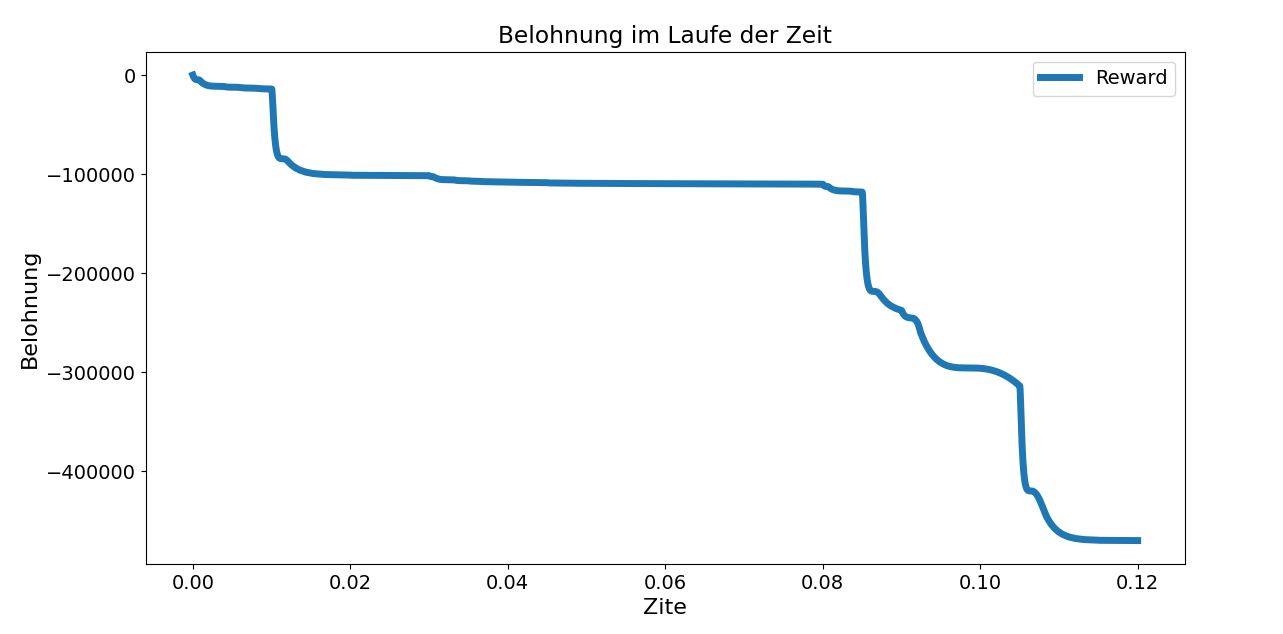
\includegraphics[width=0.99\linewidth]{3Experiment/2Experiment/4Cumulativer_Reward_Uber_Zeit.png.png}
    \caption{Kumulativer Reward über die Zeit, aufgezeichnet während der Systemtests.}
    \label{fig:CumulativeReward}
\end{figure}

\paragraph{Auswirkungen auf das Trainingsziel}
Diese Bewertungsmethodik führt zu einem quantifizierbaren Wert, der die Qualität der Regelung anzeigt und den Agenten anleitet, den Fehlerwert zu minimieren. Dies wird durch den negativen Reward widergespiegelt, der in den Lernprozess des Agenten einfließt.

\paragraph{Zeitliche Dimension der Analyse}
Selbsttests werden in wiederkehrenden Zyklen durchgeführt und bewertet, wobei der kumulierte Fehlerwert im Replay Buffer gespeichert wird, um die Strategie zu optimieren, wie in Abbildung \ref{fig:makrozyklus} illustriert.

